\section{Introduction}
\label{sec:introduction}

The goal of this laboratory assignment is to model and analyse an AC/DC converter
circuit, by designing both Envelop Detector and Voltage Regulator circuits.\par

It was chosen a full-wave bridge rectifier circuit, using 4 diodes, $D_{i={1,2,3,4}}$.
Furthermore, it was used 1 diode, $D_e$, 2 resistors, $R_e$ and $R_v$, a capacitor,
$C$, and 17 aditional diodes. The circuit described is portrayed in Figure-\ref{fig:circuit}.\par

Throughout the report it is presented a theoretical analysis, a simulation of the
circuit and its analysis as well as a comparison of the obtained results. \par

In Section~\ref{sec:analysis}, it is executed an incremental analysis by separating
the AC and DC components, in order to do a theoretical analysis of the circuit,
using the Octave maths tool.
In Section~\ref{sec:simulation}, it is executed an analysis of the circuit using
the Ngspice tool to simulate it.
In Section~\ref{sec:comparison}, reults obtained with both Octave and Ngspice are
displayed side-by-side, in order to compare the results.
Lastly, in Section~\ref{sec:conclusion}, it is performed a conclusion, bearing in mind the
results from both the theoretical analysis and the simulation, from Section~\ref{sec:analysis}
and Section~\ref{sec:simulation}, respectively.\par


\begin{figure}[h] \centering
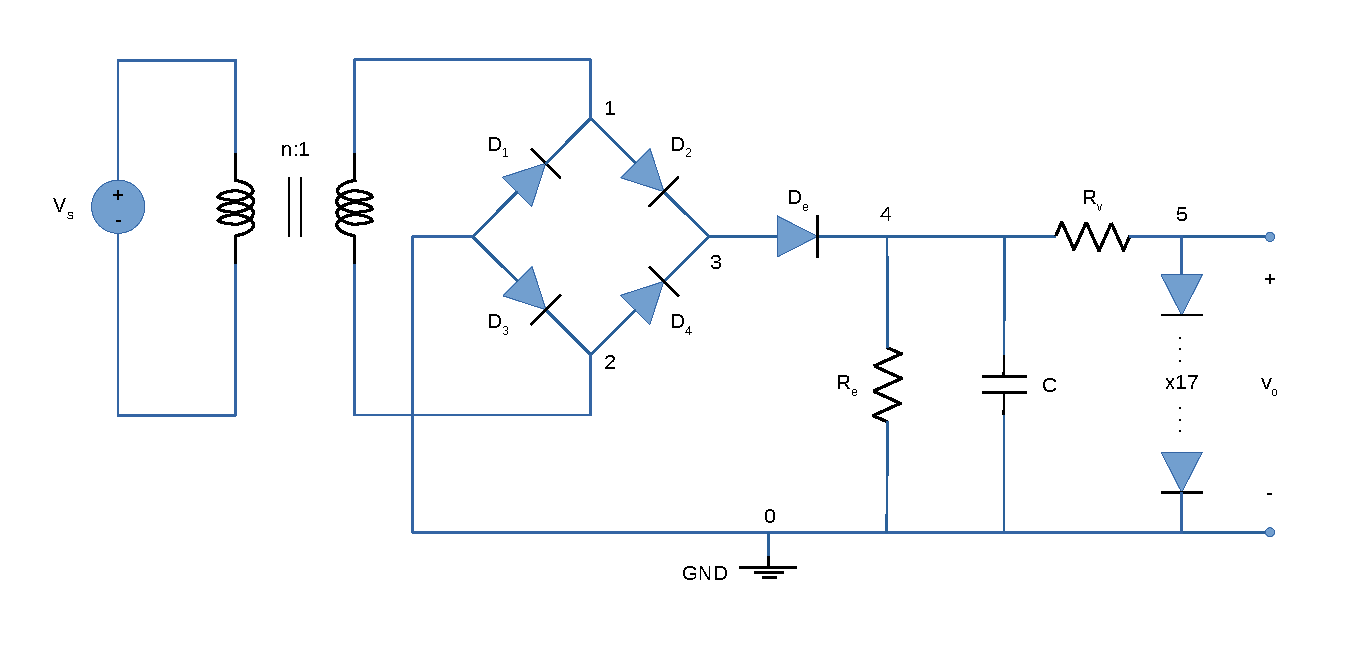
\includegraphics[width=1\linewidth]{circuit.pdf}
\caption{Circuit}
\label{fig:circuit}
\end{figure}

\newpage
